\documentclass{standalone}
% \input{/home/ai4geo/Documents/Slides/Utils/tikzzoo}

\usepackage[utf8]{inputenc}
\usepackage[T1]{fontenc}
\usepackage{tikz}
\usetikzlibrary{shapes.misc}
\usetikzlibrary{arrows.meta, quotes}
\usetikzlibrary{decorations.pathreplacing}
\usepackage{amsmath}
\usepackage{amsfonts}
\usepackage{makecell}
\usepackage{mathabx}
\usepackage{amssymb}

\definecolor{resampled}{HTML}{6096BA}
\definecolor{sunglow}{HTML}{FFD166}
\definecolor{emerald}{HTML}{5BD99E}
\definecolor{rose}{HTML}{F25584}
\definecolor{purple}{HTML}{A738EC}
\definecolor{orange}{HTML}{c17817}

\renewcommand{\familydefault}{\sfdefault}
\usetikzlibrary{shapes.misc}

\newcommand{\x}{\boldsymbol{x}}
\newcommand{\w}{\boldsymbol{w}}

\tikzset{cross/.style={cross out, draw=black, minimum size=2*(#1-\pgflinewidth), inner sep=0pt, outer sep=0pt},
%default radius will be 1pt. 
cross/.default={4pt}}
\begin{document}
  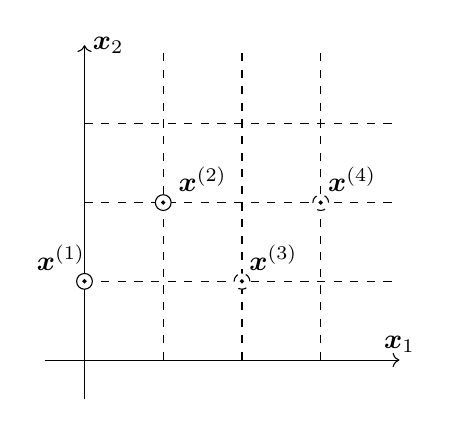
\begin{tikzpicture}

  \usetikzlibrary{calc}
  \usetikzlibrary{3d}
 
 
  \draw[->] (0, -.5) -- (0, 4);
  \draw[->] (-.5, 0) -- (4, 0);
  \draw[dashed] (1, 0) -- (1, 4);
  \draw[dashed] (2, 0) -- (2, 4);
  \draw[dashed] (3, 0) -- (3, 4);
  
  \draw[dashed] (0, 1) -- (4, 1);
  \draw[dashed] (0, 2) -- (4, 2);
  \draw[dashed] (0, 3) -- (4, 3);
  %\draw[-] (-0.5, -1.5) -- (4, 3);
  %\draw[-, dashed] (-1, -1) -- (3.5, 3.5);
  %\draw[-, dashed] (0.5, -1.5) -- (4.5, 2.5);
  %\draw[->, thick] (2, 3) -- (3, 2);
  
  \draw[fill=white, dashed](2, 1) circle (0.1);
  \draw[fill=black](2, 1) circle (0.02);
  
  \draw[fill=white, dashed](3, 2) circle (0.1);
  \draw[fill=black](3, 2) circle (0.02);
  
  %\draw[fill=white, dashed](2.5, -1.2) circle (0.1);
  %\draw[fill=black](2.5, -1.2) circle (0.02);
  
  %\draw[fill=white, dashed](2.2, -0.5) circle (0.1);
  %\draw[fill=black](2.2, -0.5) circle (0.02);
  
  %\draw[fill=white, dashed](3, 1.2) circle (0.1);
  %\draw[fill=black](3, 1.2) circle (0.02);
  
  %\draw[fill=white](3.5, 2) circle (0.1);
  %\draw[fill=black](3.5, 2) circle (0.02);
  
  %\draw[fill=white](0.6, 1) circle (0.1);
  %\draw[fill=black](0.6, 1) circle (0.02);
  
  %\draw[fill=white](1, 1.2) circle (0.1);
  %\draw[fill=black](1, 1.2) circle (0.02);
  
  \draw[fill=white](0, 1) circle (0.1);
  \draw[fill=black](0, 1) circle (0.02);
  
  \draw[fill=white](1, 2) circle (0.1);
  \draw[fill=black](1, 2) circle (0.02);

  
  %\draw[-] (-0.5, -.5) -- (4, 2);
  %\draw[-, dashed] (-0.5, -0.25) -- (4, 2.25);
  %\draw[-, dashed] (-0.5, -0.75) -- (4, 1.75);
  
  
  \node at (-0.3, 1.3) {$\x^{(1)}$};
  \node at (1.5, 2.3) {$\x^{(2)}$};
  \node at (2.4, 1.3) {$\x^{(3)}$};
  \node at (3.4, 2.3) {$\x^{(4)}$};
  %\node at (1, 2.3) {$\x^{(5)}$};

  \node at (4, 0.2) {$\x_1$};
  \node at (0.3, 4) {$\x_2$};
  
  
  \end{tikzpicture}
\end{document}
